Základní řídící jednotka je tedy schopná poskytnout základní funkce, které jsou potřeba pro většinu her.
Některé hry ale mohou vyžadovat nějakou specifickou funkci, kterou základní zařízení nedokáže poskytnout.
Proto je vhodné, aby bylo možné k~základnímu zařízení připojit externí moduly, bez kterých by se konkrétní hry neobešly.

\subsection{Modul dvířka}
Asi nejzákladnější modul jsou dvířka.
Dvířka přidávají uzamykatelné přihrádky.
Do stanoviště se tak dá uzamknout předmět potřebný ke splnění úkolu, který hráči získají například po zadání hesla nebo vyřešení zadaného úkolu.
Přihrádky pak mohou sloužit pro více týmů nebo třeba uchovávat více objektů do různých částí hry.

Pro jednoduchost jsou dvířka zamykána magneticky.
Vrátka jsou uchycena na kloubu ve své horní části a~v dolní části se nachází magnet.
Pod dnem přihrádky se pak nachází servomotor vybavený druhým magnetem, který tak může dvířka přitáhnout nebo odpudit.
Toto řešení neposkytuje bezpečné uzamčení přihrádky, vrátka se dají vypáčit někdy i~nehtem, ale pro účely her je to dostačující řešení.
Aby bylo možné ověřit, zda se vrátka dovřela, je vedle serva i~spínač, který se sepne při dovření vrátek.
Z~tohoto řešení vyplynula další možnost jak modul dvířek využít.
Vrátka se při odemčení pootevřou, a~protože jsou v~tu chvíli jen odpuzována magnetem, je možné je stlačit zpět a~sepnout tak spínač.
Tento fakt se ukázal být užitečný, protože tak vznikly velká pohodlná tlačítka.
Struktura tohoto modulu je vidět na diagramu \ref{fig:diagram_dvirka} ve verzi se čtyřmi přihrádkami.

\begin{figure}[h]
    \centering
    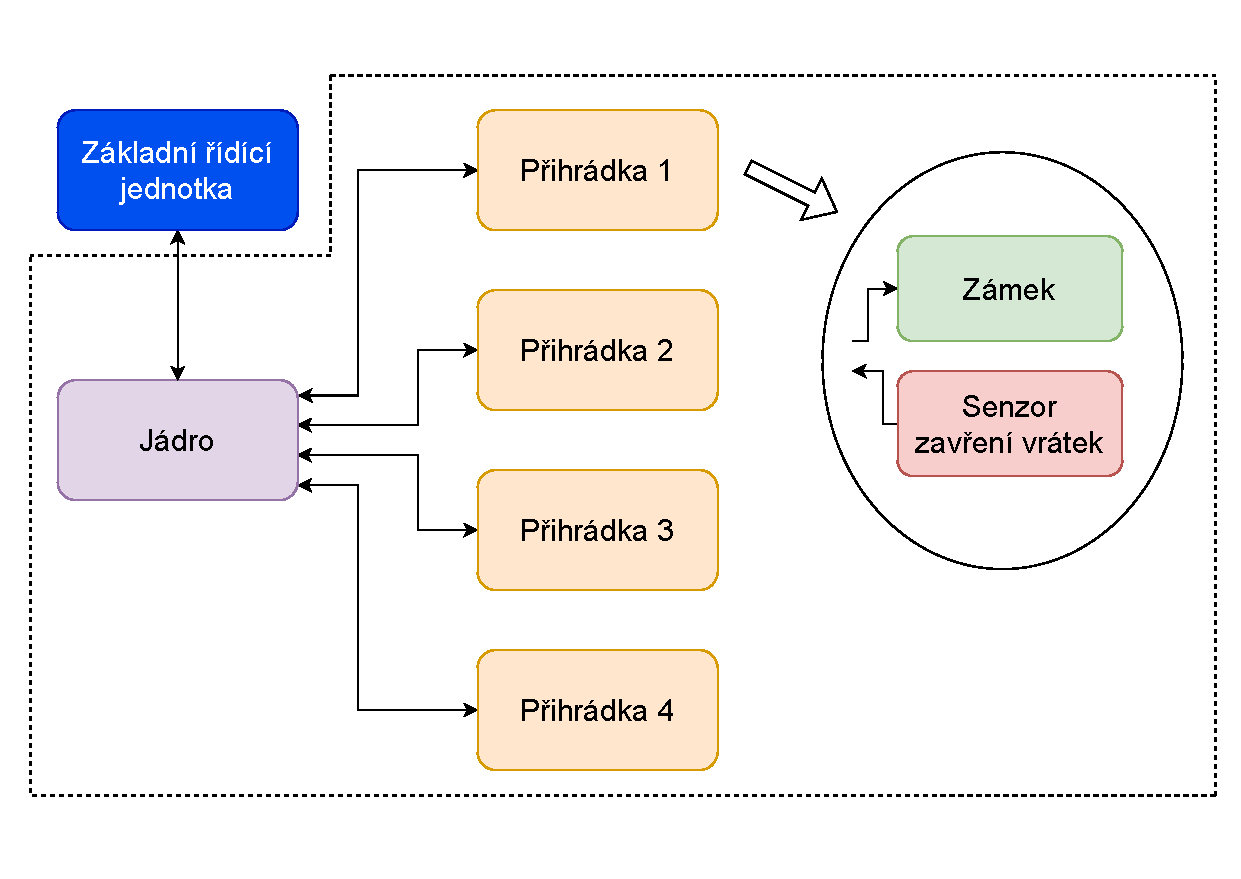
\includegraphics[width=0.65\textwidth]{text/TeoretickyUvod/AplikaceHernichZarizeni/diagram/Dvirka.drawio.pdf}
    \caption{Blokové schéma modulu dvířka}
    \label{fig:diagram_dvirka}
\end{figure}
 
Jednoduchá hra, která vyžaduje modul dvířka, je např. hra Maják. %%TODO: vymyslet lepčí název tohle se  mi moc nepozdává (je to název z~her od Petra na první lucerný v~roce 2021)
V~této hře jsou hráči rozděleni do týmů a~každý tým má svou barvu, od které je odvozena konkrétní přihrádka. 
Týmy mají za úkol získat co nejvíc sad kartiček.
Na hřišti je několik automatických stanovišť s~modulem dvířka a~v každém z~nich je nějaký typ kartičky.
Každé stanoviště během hry umožňuje přístup vždy právě jednomu z~týmů, který v~pravidelném intervalu mění a~čas do změny reprezentuje na jednom z~kruhů.
Při startu hry si každé stanoviště náhodně vybere tým, kterým začne, a~následně se už drží konstantního pořadí.
Když někdo dorazí ke stanovišti ve chvíli, kdy je stanoviště zpřístupněné jeho týmu, a~klepne na tlakovou plochu, stanoviště mu vydá kartičku.
Stanoviště se týmu zpřístupní jen v~čase daného týmu a~navíc jen jednou za kolo.
Hráčům cíleně není představen celý mechanizmus výdeje kartiček, je jim řečeno jen, že se přihrádka otevírá klepnutím do tlakové plochy a~že je zajímají jen kartičky jejich barvy. 
Tým tedy musí spolupracovat nejprve na odhalení mechanizmu a~následně myslet jak zvítězit.

Podobná hra se buď dá hrát samostatně nebo může jít například jen o~metodu, jak získávat suroviny v~nějaké komplexnější hře.

\subsection{Zvukový modul}
Další plánovaný modul, který se dá připojit, je zvukový modul.
Hra, která vyžaduje zvukový modul, je například hra s~názvem Ticho.
Tato hra vyžaduje zároveň i~modul dvířka.
V~této hře stanoviště sleduje intenzitu zvuku v~okolí a~v momentě, kdy hluk klesne pod stanovenou úroveň, stanoviště otevře dvířka. 
% Ucastnikum není ovládání představeno a~musí tak na něj přijít samy.
Stanoviště je hráčům představeno jako "magická krabička" za čárou, ke které se nesmí proplížit, ale můžou ji ovlivnit z~dálky.
Úkolem hráčů tak je přijít na to, jak krabička funguje a~jak ji přesvědčí, aby se otevřela.

V~rámci zvukového modulu je i~možnost nahrávku přehrát.
Tato část zvukového modulu umožňuje intenzivnější vtažení hráče do hry s~příběhem.
Může jít například o~únikovou hru, při které se hráč ocitne v~oblasti neznámého bludiště a~jeho úkolem je najít cestu ven.
Při hledání může narazit na různá stanoviště, která mu nejprve přehrají nějakou část příběhu a~následně mu dají úkol nebo radu jak postupovat dál.

Podstatným modulem je také komunikační modul, který umožňuje připojení k~mobilní síti a~tím i~komunikaci s~ostatními zařízeními na velkou vzdálenost.
Tento modul je potřeba například pro hru Zábor kopce.

V~této hře se na hřišti o~velké rozloze nachází několik automatických stanovišť.
Hráči jsou rozděleni do týmů a~každý tým má svou barvu a~své tlačítko na stanovišti označené barvou týmu.
V~hře Zábor Kopce je hlavním cílem získávat body pro svůj tým ovládnutím a~udržením stanovišť na rozsáhlém hřišti. 
Axiální světelný kruh zobrazuje rozdělení tlakové plochy na jednotlivá tlačítka týmů podle jejich barvy.
Zabrání stanoviště pak mohou hráči provést stiskem příslušného tlačítka. 
Získávání bodů se odehrává dvěma způsoby, ovládnutím stanoviště a~následným držením stanoviště pod kontrolou. 
Týmy mohou přebírat stanoviště od soupeřů, což přidává hře strategický rozměr. 
Výhodou je kontrolovat více stanovišť najednou, což umožňuje rychlejší získávání bodů a~zvyšuje šanci na vítězství.
Komunikační modul je tu potřebný pro vyhodnocování hry.
Stanoviště totiž musí být schopné komunikovat s~centrálním serverem, který vyhodnocuje hru a~zobrazuje její průběh.
Tato hra je původně navržena pro airsoftové hráče na hřiště v~Mokra-Horakov o~rozloze \(6.7\-[ha]\) \cite{MokraHorakov}.
V~takovém prostředí tedy komunikace pomocí WiFi či Bluetooth nedostačuje, protože stanoviště mohou být i~několik set metrů od sebe.

\subsection{Výběr bezdrátové komunikace dlouhého dosahu}
Pro komunikaci na vzdálenosti v~řádu jednotek kilometrů se nabízí asi jen dvě základní možnosti, LoRa a~mobilní síť.
Ještě počátkem roku 2023 by byla i~třetí možnost, Sigfox, ale jeho síť byla v~ČR vypnuta \cite{SigfoxKonci}.

LoRa je technologie určená pro komunikaci na dlouhé vzdálenosti s~malou spotřebou a~datovou propustností.
Pracuje v~bezlicenčním pásmu a~není tedy třeba platit za provoz.
Její dosah je i~v zastavěné oblasti v~řádu kilometrů \cite{LoRaSEMTECH}, a~za ideálních podmínek na přímou viditelnost i~přes sto kilometrů \cite{LoRaEMAN}. 
Nevýhoda LoRy je ale malá datová propustnost ještě snížená omezením času provozu na \(1\-\%\)\cite{LoRaEMAN}.

Mobilní síť má v~porovnání s~LoRou výrazně větší datovou propustnost, ale na druhou stranu je třeba platit za provoz a~je méně energeticky úsporná.
Například NB-IoT je energeticky asi o~třetinu náročnější než LoRa.
Přesto je dostatečně úsporná, aby bylo zařízení, které tuto technologii využívá, schopno běžet na baterii přes deset let \cite{LoRaVSNB-IoT}.
Energetická náročnost tedy není problém a~vyšší datová propustnost společně s~připojením na internet je významnější výhoda než bezplatný provoz u~LoRy.
Další výhodou LoRy by mohla být nezávislost na pokrytí mobilních sítí, ale vzhledem k~tomu, že pokrytí NB-IoT sítě je v~ČR údajně \(100\-\%\)\cite{NB-IoTPokryti}, není tento fakt důležitý. 
